\documentclass{article}

%% Created with wxMaxima 12.01.0

\setlength{\parskip}{\medskipamount}
\setlength{\parindent}{0pt}
\usepackage[utf8]{inputenc}
\usepackage{graphicx}
\usepackage{color}
\usepackage{amsmath}

\definecolor{labelcolor}{RGB}{100,0,0}

\begin{document}

\noindent
%%%%%%%%%%%%%%%
%%% INPUT:
\begin{minipage}[t]{8ex}{\color{red}\bf
\begin{verbatim}
(%i223) 
\end{verbatim}}
\end{minipage}
\begin{minipage}[t]{\textwidth}{\color{blue}
\begin{verbatim}
E:180;
Vm:230*sqrt(2),numer;
a:108*%pi/180;
R:12;
L:22*10^-3;
f:50;
T:1/f;
w:f*2*%pi,numer;
b:atan(w*L/R),numer;
z:sqrt(R^2+(w*L)^2),numer;
V(t):=Vm*sin(w*t+a);
C:(E/R)-Vm/z*sin(a-b),numer;
ti:-0.001;
tf:0.02;
\end{verbatim}}
\end{minipage}
%%% OUTPUT:
\begin{math}\displaystyle
\parbox{8ex}{\color{labelcolor}(\%o223) }
180
\end{math}

\begin{math}\displaystyle
\parbox{8ex}{\color{labelcolor}(\%o224) }
325.2691193458119
\end{math}

\begin{math}\displaystyle
\parbox{8ex}{\color{labelcolor}(\%o225) }
\frac{3\,\pi }{5}
\end{math}

\begin{math}\displaystyle
\parbox{8ex}{\color{labelcolor}(\%o226) }
12
\end{math}

\begin{math}\displaystyle
\parbox{8ex}{\color{labelcolor}(\%o227) }
\frac{11}{500}
\end{math}

\begin{math}\displaystyle
\parbox{8ex}{\color{labelcolor}(\%o228) }
50
\end{math}

\begin{math}\displaystyle
\parbox{8ex}{\color{labelcolor}(\%o229) }
\frac{1}{50}
\end{math}

\begin{math}\displaystyle
\parbox{8ex}{\color{labelcolor}(\%o230) }
314.1592653589793
\end{math}

\begin{math}\displaystyle
\parbox{8ex}{\color{labelcolor}(\%o231) }
0.5225544346474
\end{math}

\begin{math}\displaystyle
\parbox{8ex}{\color{labelcolor}(\%o232) }
13.84806431604333
\end{math}

\begin{math}\displaystyle
\parbox{8ex}{\color{labelcolor}(\%o233) }
\mathrm{V}\left( t\right) :=Vm\,\mathrm{sin}\left( w\,t+a\right) 
\end{math}

\begin{math}\displaystyle
\parbox{8ex}{\color{labelcolor}(\%o234) }
-7.980226969896119
\end{math}

\begin{math}\displaystyle
\parbox{8ex}{\color{labelcolor}(\%o235) }
-0.001
\end{math}

\begin{math}\displaystyle
\parbox{8ex}{\color{labelcolor}(\%o236) }
0.02
\end{math}
%%%%%%%%%%%%%%%


\noindent
%%%%%%%%%%%%%%%
%%% INPUT:
\begin{minipage}[t]{8ex}{\color{red}\bf
\begin{verbatim}
(%i237) 
\end{verbatim}}
\end{minipage}
\begin{minipage}[t]{\textwidth}{\color{blue}
\begin{verbatim}
i(t):=C*%e^(-R/(L)*t)+Vm/z*sin(w*t+a-b)-(E/R);
Vt(t):=if i(0)>=0 and i(t)>0 and t<T/2 then V(t) else 0;
wxplot2d([i(t)],[t,ti,tf],[y,-40,10],[gnuplot_preamble, "set grid"]);
\end{verbatim}}
\end{minipage}
%%% OUTPUT:
\begin{math}\displaystyle
\parbox{8ex}{\color{labelcolor}(\%o237) }
\mathrm{i}\left( t\right) :=C\,{e}^{\frac{-R}{L}\,t}+\frac{Vm}{z}\,\mathrm{sin}\left( w\,t+a-b\right) -\frac{E}{R}
\end{math}

\begin{math}\displaystyle
\parbox{8ex}{\color{labelcolor}(\%o238) }
\mathrm{Vt}\left( t\right) :=\mathrm{if} \mathrm{i}\left( 0\right) >=0 and \mathrm{i}\left( t\right) >0 and t<\frac{T}{2} \mathrm{then} \mathrm{V}\left( t\right)  \mathrm{else} 0
\end{math}

\begin{math}\displaystyle
\parbox{8ex}{\color{labelcolor}(\%t239) }
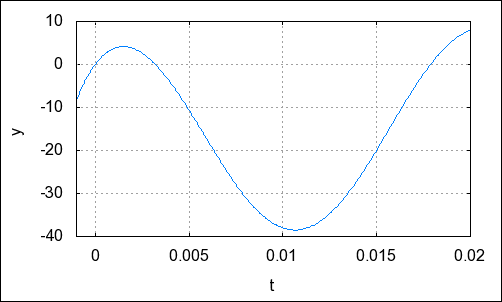
\includegraphics[width=9cm]{problema_2_8_img/problema_2_8_1.png}
\end{math}

\begin{math}\displaystyle
\parbox{8ex}{\color{labelcolor}(\%o239) }

\end{math}
%%%%%%%%%%%%%%%


\noindent
%%%%%%%%%%%%%%%
%%% INPUT:
\begin{minipage}[t]{8ex}{\color{red}\bf
\begin{verbatim}
(%i240) 
\end{verbatim}}
\end{minipage}
\begin{minipage}[t]{\textwidth}{\color{blue}
\begin{verbatim}
wxplot2d([V(t), Vt(t)],[t,ti,tf],[y,-350,350],[gnuplot_preamble, "set grid"]);
\end{verbatim}}
\end{minipage}
%%% OUTPUT:
\begin{math}\displaystyle
\parbox{8ex}{\color{labelcolor}(\%t240) }
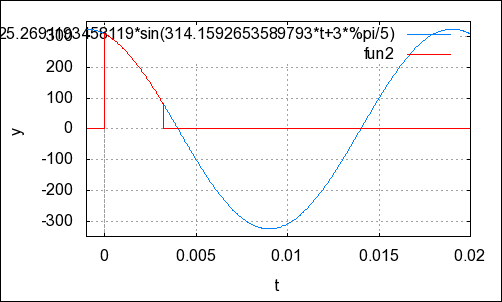
\includegraphics[width=9cm]{problema_2_8_img/problema_2_8_2.png}
\end{math}

\begin{math}\displaystyle
\parbox{8ex}{\color{labelcolor}(\%o240) }

\end{math}
%%%%%%%%%%%%%%%


\noindent
%%%%%%%%%%%%%%%
%%% INPUT:
\begin{minipage}[t]{8ex}{\color{red}\bf
\begin{verbatim}
-->  
\end{verbatim}}
\end{minipage}
\begin{minipage}[t]{\textwidth}{\color{blue}
\begin{verbatim}
kill(all);
\end{verbatim}}
\end{minipage}
%%% OUTPUT:
\begin{math}\displaystyle
\parbox{8ex}{\color{labelcolor}(\%o0) }
done
\end{math}
%%%%%%%%%%%%%%%


\noindent
%%%%%%%%%%%%%%%
%%% INPUT:
\begin{minipage}[t]{8ex}{\color{red}\bf
\begin{verbatim}
-->  
\end{verbatim}}
\end{minipage}
\begin{minipage}[t]{\textwidth}{\color{blue}
\begin{verbatim}
val(t):=Vm*sin(w*t);
\end{verbatim}}
\end{minipage}
%%% OUTPUT:
\begin{math}\displaystyle
\parbox{8ex}{\color{labelcolor}(\%o18) }
\mathrm{val}\left( t\right) :=Vm\,\mathrm{sin}\left( w\,t\right) 
\end{math}
%%%%%%%%%%%%%%%


\noindent
%%%%%%%%%%%%%%%
%%% INPUT:
\begin{minipage}[t]{8ex}{\color{red}\bf
\begin{verbatim}
-->  
\end{verbatim}}
\end{minipage}
\begin{minipage}[t]{\textwidth}{\color{blue}
\begin{verbatim}
ev(val(t),t=0.006);
\end{verbatim}}
\end{minipage}
%%% OUTPUT:
\begin{math}\displaystyle
\parbox{8ex}{\color{labelcolor}(\%o27) }
309.3493155034204
\end{math}
%%%%%%%%%%%%%%%

\end{document}
